\documentclass[../main.tex]{subfiles}

\graphicspath{{../images/}}

\begin{document}
\pagestyle{fancy}
\lhead{Lecture 11: 10/1/24}
\chead{Chapter 4}
\rhead{PHYS 421}

\section{Electric Fields in Matter}
\barh \vspace{1em}

\subsection{Polarization} 

\subsubsection{Dielectrics}

In dieletrics, ``All charges are attached to specific atoms or molecules'' (Griffith, pg.166)

\subsubsection{Induced Dipoles}

% fig4_1_2.png
\begin{figure*}[ht]
    \centering
    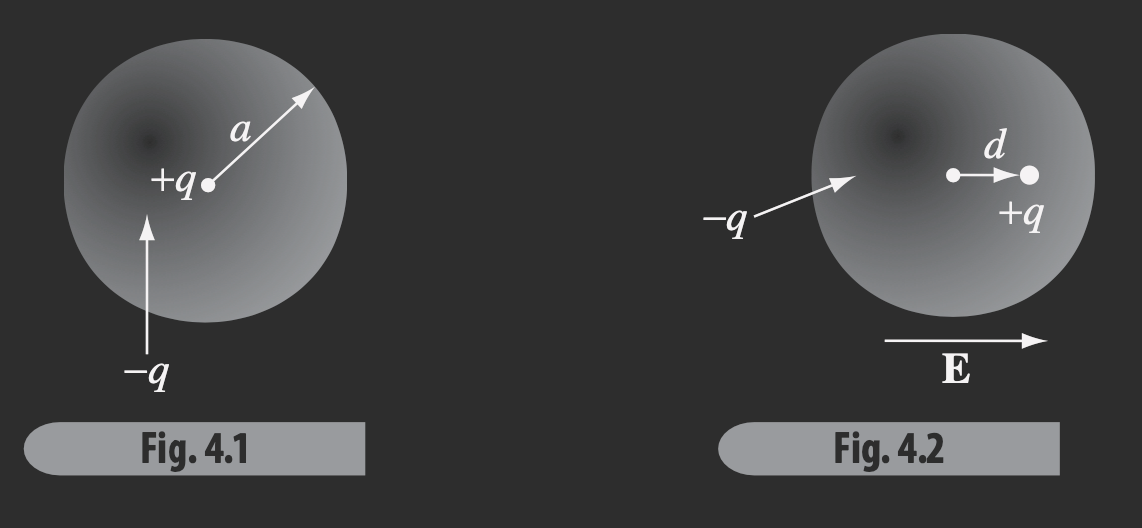
\includegraphics[width=0.5\linewidth]{fig4_1_2.png}
    \caption{Left: Simple Nucleus $+q$ surrounded by spherical cloud $-q$ of radius $a$. Right: In an external electric field $E$ the nucleus shifts right $d$ and the cloud shifts left.}
    \label{fig:4_1_2}
\end{figure*}

For a simple model of the atom (Fig. \ref{fig:4_1_2}), the electric field at $d$ is
\begin{align*}
    E_d = \ke \frac{qd}{a^3}
\end{align*}
where the dipole moment is $p = qd$. We have equilibrium when
\begin{align*}
    F_\text{ext} = q E_\text{ext} = q_- E_d
\end{align*}
So using the dipole moment 
\begin{align*}
    \abs{\vb p} = qd = 4\pi \epsilon_0 a^3 E_\text{ext} = \alpha E_\text{ext} 
\end{align*}
Here we have this ``atomic polaritability''
\begin{align*}
    \alpha = 4\pi \epsilon_0 a^3 = 3\epsilon v
\end{align*}
where $v$ is the volume of the atom. Comment: this crude approximation is still accurate by a factor of 4.

In general we have a vector
\begin{align*}
    \vb p = \hat \alpha \vb E
\end{align*}
where $\hat \alpha$ is the polarizability tensor. For a linear dielectric relation between $E$ and $p$ we get
\begin{align*}
    \hat \alpha = \begin{bmatrix}
        \alpha_{xx} & \alpha_{xy} & \alpha_{xz} \\
        \alpha_{yx} & \alpha_{yy} & \alpha_{yz} \\
        \alpha_{zx} & \alpha_{zy} & \alpha_{zz}
    \end{bmatrix}
\end{align*}

\subsubsection{Alignment of Polar Molecules}

The dipole will experience a torque in and $E$-field
\begin{align*}
    \vb N &= (\vb r_+ \cross \vb F_+) + (\vb r_- \cross \vb F_-) \\
    &= \qt(\frac{\vb d}{2} \cross q\vb E) + \qt(-\frac{\vb d}{2} \cross q\vb E) \\
    &= q \vb d \cross \vb E
\end{align*}
thus
\begin{align*}
    \vb N = \vb p \times \vb E
\end{align*}
which implies that there is a force that acts to align $\vb p \parallel \vb E$.

\paragraph{WHat if E is not uniform?}
\begin{align*}
    \vb F = \vb F_+ + \vb F_- = q \vb E + q \vb E = q \Delta E
\end{align*}
assuming small $d$ in $E_x$, then
\begin{align*}
    \Delta E_x = (\grad \vb E_x) \cdot \vb d
\end{align*}
So the total change in the field is
\begin{align*}
    \Delta \vb E = (\vb d \cdot \grad) \vb E
\end{align*}
thus
\begin{align*}
    \vb F = (\vb p \cdot \grad) \vb E
\end{align*}

\begin{figure*}[ht]
    \centering
    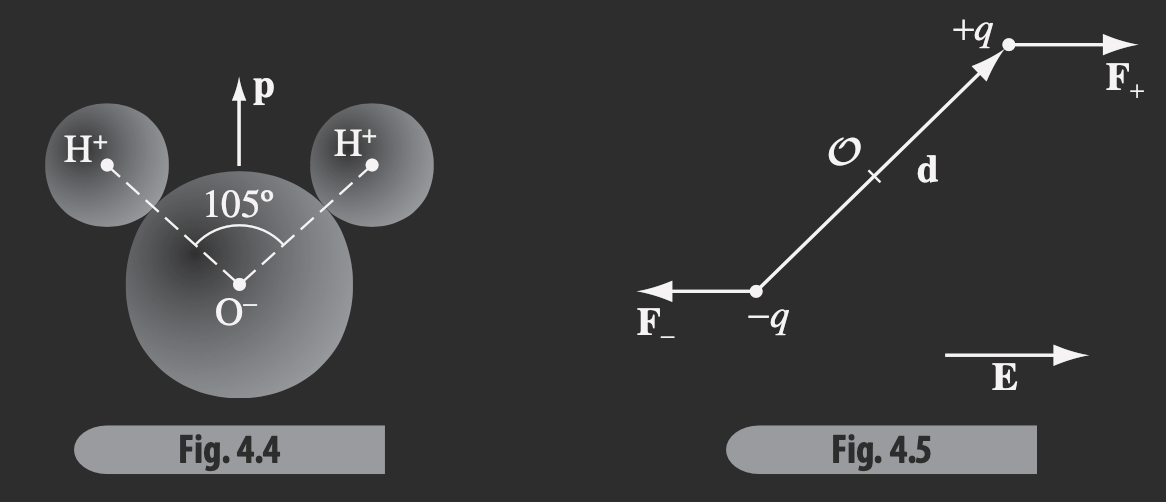
\includegraphics[width=0.5\linewidth]{fig4_4_5.png}
    \caption{Dipole moment in oxygen molecule, and in an electric field.}
    \label{fig:4_4_5}
\end{figure*}

\paragraph{Example:} Problem 4.5
\begin{figure*}[ht]
    \centering
    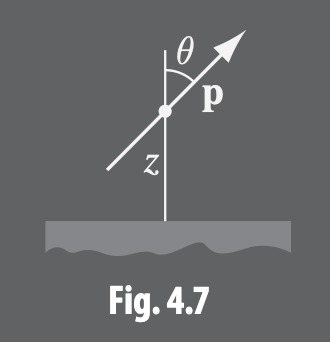
\includegraphics[width=0.3\linewidth]{fig4_7.png}
    \caption{Infinitely grounded conductor with dipole at an angle $\theta$ from the normal plane and nailed in place.}
    \label{fig:fig4_7}
\end{figure*}
Using the method of images % fig4_7a.png and fig4_7b.png
\begin{figure*}
    \centering
    \begin{tabular}{c c}
        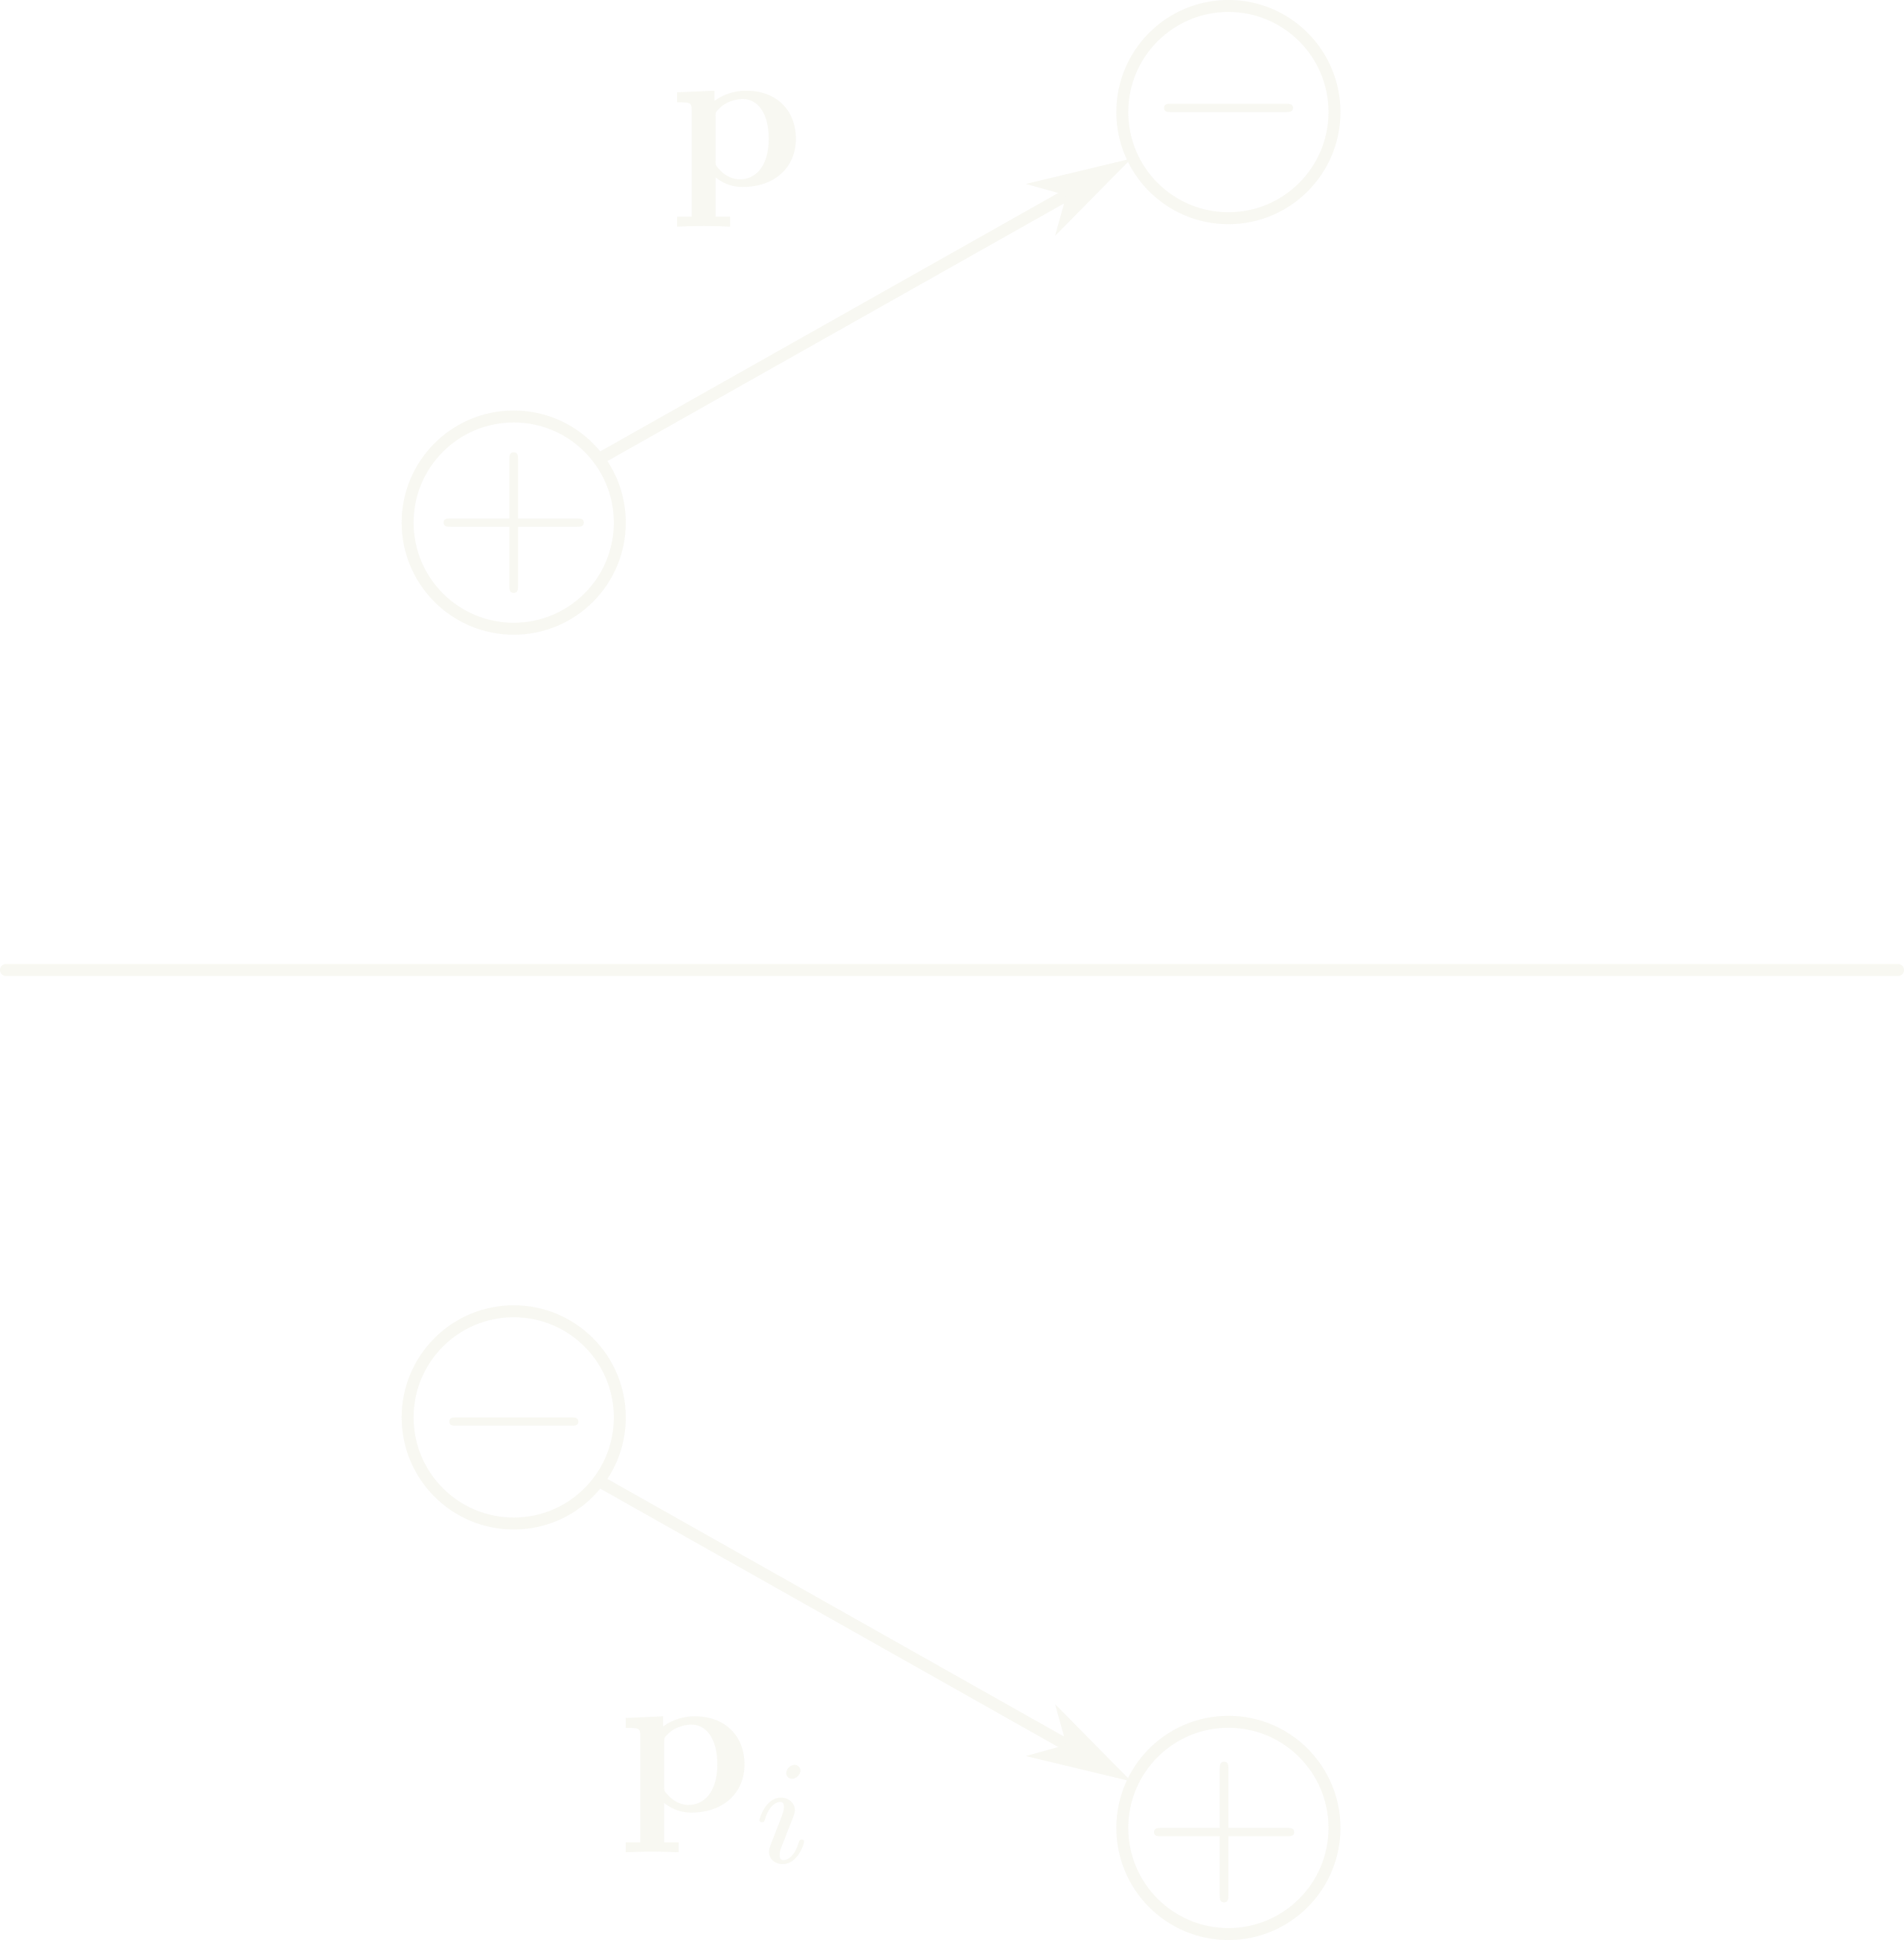
\includegraphics[width=0.3\linewidth]{fig4_7a.png} & 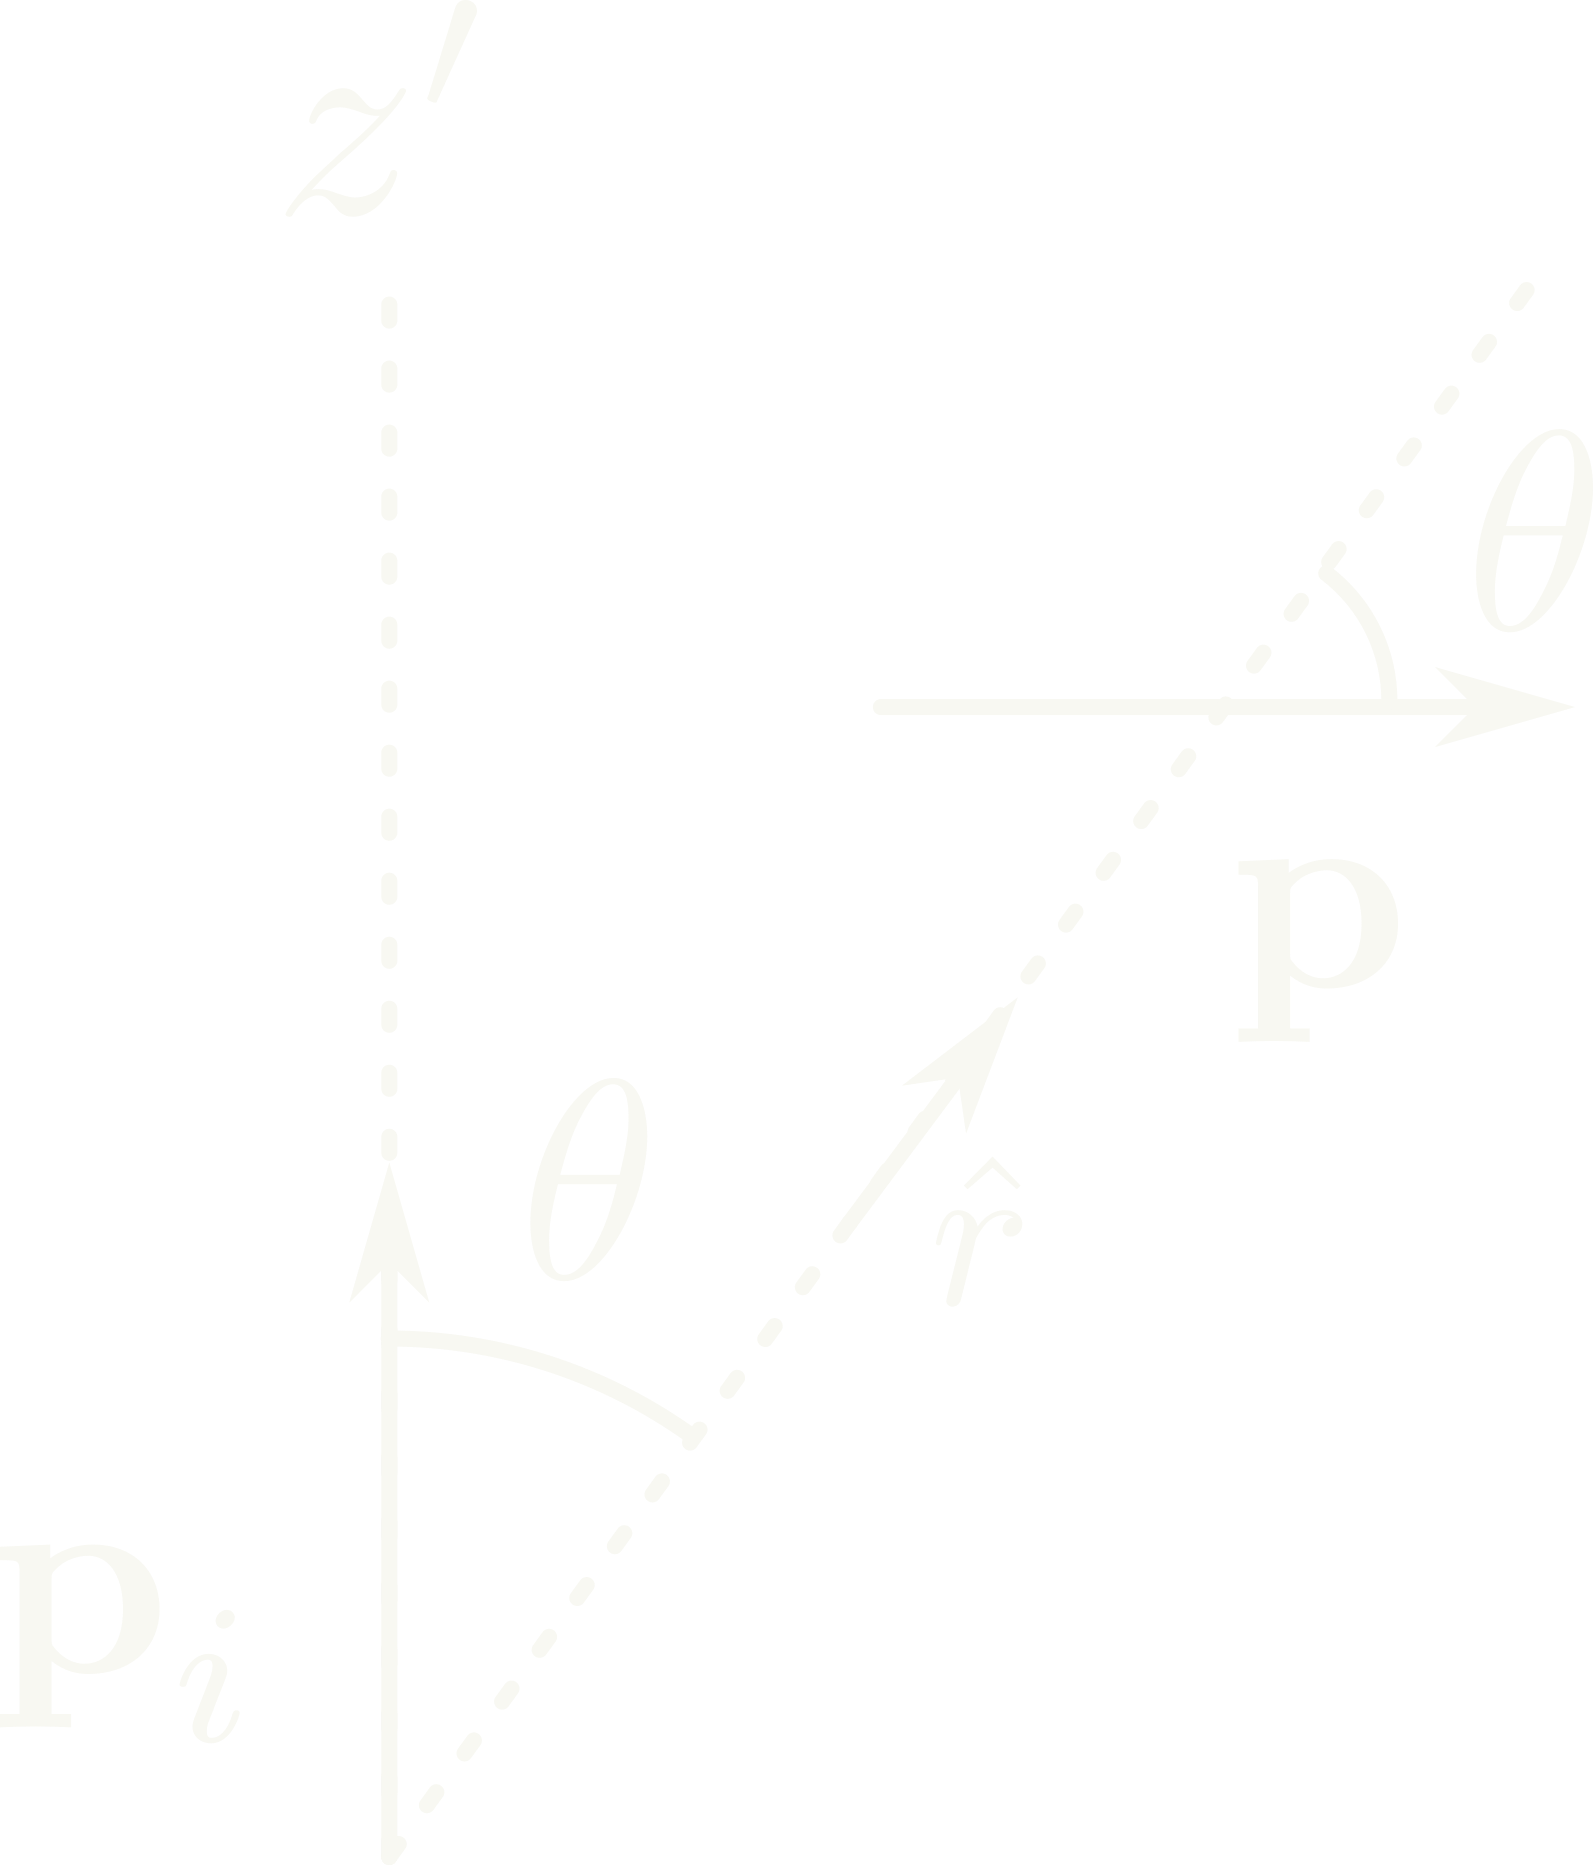
\includegraphics[width=0.3\linewidth]{fig4_7b.png}
    \end{tabular}
    \caption{Left: Method of images using image dipole. Right: Coordinate using image dipole up as $z'$.}
\end{figure*}

Where look at $\vb p_i$ coordinate (pointing up) thus $2z$ away we have the dipole pointing perpendicular to the image dipole i.e.
\begin{align*}
    \vb E_i = \ke \frac{p_i}{r^3} \qt(
        2\cos\theta \vu r + \sin\theta \vu \theta
    )
\end{align*}
where
\begin{align*}
    \vb p = p\cos\theta \vu r + p\sin\theta \vu \theta
\end{align*}
So the torque $\vb N = \vb p \cross \vb E_i$ is
\begin{align*}
    \vb N &= \ke \frac{p^2}{(2z)^3} (\cos\theta \vu r + \sin\theta \vu \theta) \cross \qt(
        2\cos\theta \vu r + \sin\theta \vu \theta
    ) \\
    &= \ke \frac{p^2}{(2z)^3} \qt(
        \cos\theta \sin\theta \vu*\phi + 2\cos\theta\sin\theta (-\vu*\phi)
        ) \\
    &= \ke \frac{p^2 \cos\theta\sin\theta}{(2z)^3} (-\vu*\phi) \\
    &= \ke \frac{p^2 \sin(2\theta)}{8\pi \epsilon_0 (8z^3)} (-\vu*\phi)
\end{align*}
So
\begin{align*}
    \begin{cases}
        0 < \theta < \frac{\pi}{2} & N\sim -\vu*\phi \\
        \frac{\pi}{2} < \theta < \pi & N\sim \vu*\phi
    \end{cases}
\end{align*}
Which means the dipole can either align perdendicularly up or down depending on the angle $\theta$.

\subsubsection{Polarization}
\begin{align*}
    \vb P \equiv \textrm{dipole moment per unit volume}
\end{align*}
i.e. the little $\vb p$ is
\begin{align*}
    \vb p = \vb P \dd\tau
\end{align*}

\subsection{The Field of a Polarized Object}
\subsubsection{Bound Charges}

For a single dipole
\begin{align*}
    V_\text{dip}(\vb r) = \ke \frac{\vb p \cdot \vu \scriptr}{\scriptr^2}
\end{align*}
and using the dipole moment per unit volume def:
\begin{align*}
    V_\text{dip}(\vb r) = \ke \int \frac{\vb P(\vb r') \cdot \vu \scriptr}{\scriptr^2} \dd\tau'
\end{align*}
recalling the math fact
\begin{align*}
    \grad' \qt(\frac{1}{\scriptr}) = \frac{\vu \scriptr}{\scriptr^2}
\end{align*}
thus
\begin{align*}
    V &= \ke \int \vb P(\vb r') \cdot \grad' \qt(\frac{1}{\scriptr}) \dd\tau'
\end{align*}
using another math fact
\begin{align*}
    \div (F \vb A) = F(\div \vb A) + \vb A \cdot (\grad F)
\end{align*}
So we can rewrtite the integral
\begin{align*}
    V &= \ke \qt[
        \int_V \div(\frac{\vb P}{\scriptr}) \dd\tau' - \int_V \frac{1}{\scriptr} \div \vb P \dd\tau'
    ] \\
    &= \ke \qt[
        \oint_S \frac{1}{\scriptr} \vb P \cdot \dd \vb a' - \int_V \frac{1}{\scriptr} \div \vb P \dd\tau'
    ]
\end{align*}
where we used the divergence theorem for the first term. For charge densities
\begin{align*}
    \begin{cases}
        \textrm{surface charge} & \sigma_b \equiv \vb P \cdot \vu n \\
        \textrm{volume charge} & \rho_b \equiv -\div \vb P
    \end{cases}
\end{align*}
then
\begin{align*}
    V = \ke \qt[
        \oint_S \frac{\sigma_b}{\scriptr} \dd a' + \int_V \frac{\rho_b}{\scriptr} \dd\tau'
    ]
\end{align*}

\subsubsection{Physical Interpretation of Bound Charges}
So for a charge neutral sphere with an applied $E$-field, we can imagine this sphere as two oppositely charge spheres superimposed on each other but slighly shifted (Fig. \ref{fig:4_15}).
\begin{figure*}[ht]
    \centering
    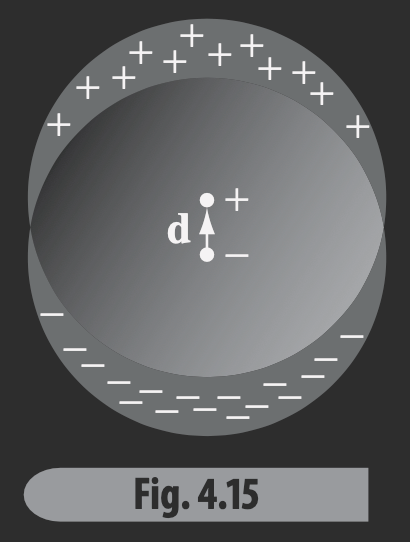
\includegraphics[width=0.3\linewidth]{fig4_15.png}
    \caption{Charge neutral sphere with applied $E$-field.}
    \label{fig:4_15}
\end{figure*}
Thus we can imagine a collection of dipoles for each atom in a material with alternating charges.
This is actually wrong (read Berry Phases in Electronic Structure Theory by David Vanderbilt).

\newpage
\lhead{Lecture 12: 10/3/24}
\paragraph{Example:} Find $\vb E$ of a uniformly polarized sphere of radius $R$.

\begin{figure*}[ht]
    \centering
    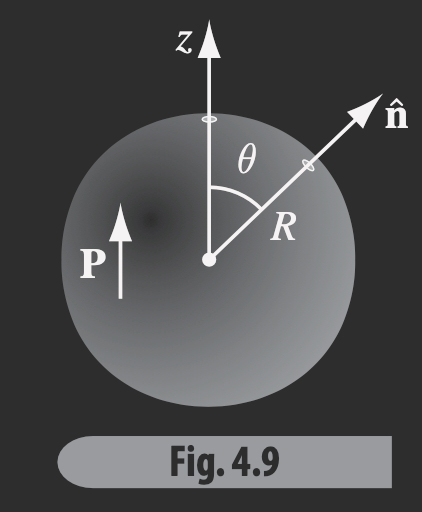
\includegraphics[width=0.2\linewidth]{fig4_9.png}
    \caption{Uniformly polarized sphere of radius $R$.}
    \label{fig:4_9}
\end{figure*}

We choose $\vb P \propto \vu z$ as shown in Fig. \ref{fig:4_9}. The bound volume and surface charges are 
\begin{align*}
    \rho_b = -\div \vb P = 0 \qqtext{but} \sigma_b = \vb P \cdot \vu n = P \cos\theta
\end{align*}
Thus using the result from before
\begin{align*}
    V = \ke \qt[
        \oint_S \frac{\sigma_b}{\scriptr} \dd a' + \int_V \frac{\rho_b}{\scriptr} \dd\tau'
    ]
\end{align*}
or 
\begin{align*}
    V(r \theta) = \begin{cases}
        \frac{P}{3\epsilon_0} r \cos\theta & r \leq R \\
        \frac{P}{3\epsilon_0} \frac{R^3}{r^2} \cos\theta & r > R
    \end{cases}
\end{align*}
Recalling $z = r \cos\theta \quad \vb E = -\grad V$ we get
\begin{align*}
    \vb E_\text{in} &= -\frac{P}{3\epsilon_0} \vu z = -\frac{1}{3\epsilon_0} \vb P
\end{align*}
and for outside the potential is
\begin{align*}
    V_\text{out} = \ke \frac{\vb p \cdot \vu r}{r^2}
\end{align*}
with the total dipole moment
\begin{align*}
    \vb p = \frac{4\pi}{3} R^3 \vb P
\end{align*}

\begin{figure*}[ht]
    \centering
    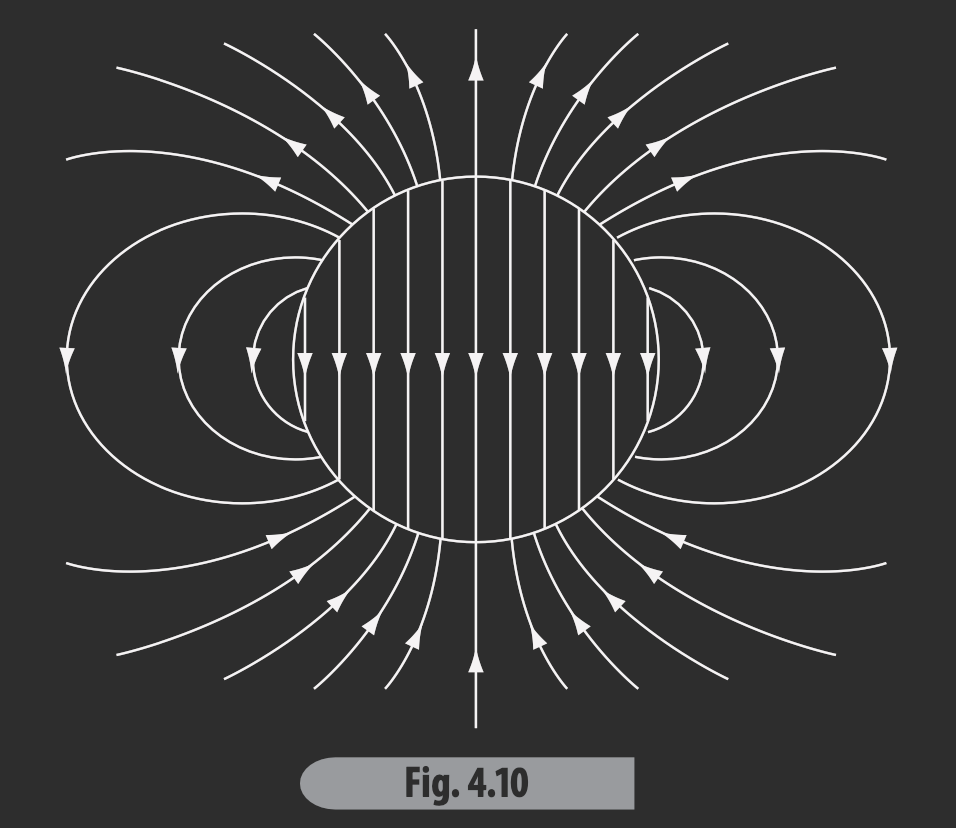
\includegraphics[width=0.3\linewidth]{fig4_10.png}
    \caption{Polarized sphere in an external $E$-field.}
    \label{fig:4_10}
\end{figure*}

So the polarized sphere is similar to the spherical conductor but with $E$-fields inside it (Fig. \ref{fig:4_10}).

\subsection{The Displacement Field}
\begin{align*}
    \rho_b = -\div \vb P \qand \sigma_b = \vb P \cdot \vu n
\end{align*}
The $\rho_\text{free} \to$ anything \textit{not} due to Polarization
\begin{align*}
    \rho = \rho_b + \rho_f
\end{align*} 
and from Gauss' Law
\begin{gather*}
    \div \vb E = \frac{\rho}{\epsilon_0} \\
    \implies \epsilon_0 \div \vb E = \rho_b + \rho_f = - \div \vb P + \rho_f
\end{gather*}
where $\vb E$ is the total electric field. Moving some terms around we get
\begin{align*}
    \div \qt(\epsilon_0 \vb E + \vb P) = \rho_f
\end{align*}
where we now define the electric displacement field
\begin{align*}
    \vb D \equiv \epsilon_0 \vb E + \vb P
\end{align*}
which has the same laws as $\vb E$:
\begin{align*}
    \boxed{\div \vb D = \rho_f} \qquad \boxed{\oint \vb D \cdot \dd\vb a = Q_\text{f, enc}}
\end{align*}

\paragraph{Example:} Long straight wire, with unform $\lambda$ (charge per length),
surrounded by rubber insulation out to radius $a$; Find $\vb D$

Using the Gaussian surface (cylinder) of length $l$ and radius $s$ so the enclosed charge is
\begin{gather*}
    \oint \vb D \cdot \dd\vb a = 2\pi s l \vb D = \lambda l \\
    \vb D = \frac{\lambda}{2\pi s} \vu s
\end{gather*}
$\implies$ holds for both $s \leq a$ and $s > a$. 

For $s > a$
\begin{align*}
    \vb P_\text{out} = 0 \implies \vb E = \frac{\vb D}{\epsilon_0} = \frac{\lambda}{2\pi \epsilon_0 s} \vu s
\end{align*}
But for inside $s \leq a$ we can't determine $\vb P_\text{in}$ yet!

\paragraph{Comments} While the two equations
\begin{align*}
    \div \vb D = \rho_f \qand \div \vb E = \frac{\rho}{\epsilon_0}
\end{align*}
are similar, the $E$-field has a Coulomb law 
\begin{align*}
    \vb E = \ke \frac{q}{\scriptr^2} \vu \scriptr
\end{align*}
but there is no equivalent for $\vb D$
\begin{align*}
    \cancel{\vb D = \ke \frac{q}{\scriptr^2} \vu \scriptr}
\end{align*}
since there is this tensor relation $\vb p = \hat \alpha \vb E$.
Furthermore, the curl is also different:
\begin{align*}
    \curl \vb D = \curl (\epsilon_0 \vb E + \vb P) = \cancel{\epsilon_0 \curl \vb E} + \curl \vb P
\end{align*}
since $\curl \vb E = \curl (-\grad V) = 0$.

\paragraph{What is D?} Units $\si{\frac{C}{m^2}}$ which is the same as $\sigma$ (surface charge density).

\subsection{Linear Dielectrics}

\subsubsection{Susceptibility, Permittivity, and Dielectric constant}
\begin{align*}
    \vb P = \epsilon_0 \chi_e \vb E
\end{align*}
where $\chi_e$ is the electric susceptibility (dimensionless). For here, we will assume linear (isotropic \& homogeneous) dielectrics.
\begin{itemize}
    \item vacuum: $\chi_e = 0$
    \item air: $1.00054$
    \item salt: $\sim 4.9$
    \item Si: $\sim 11$
    \item water: $\sim 80$ (water is already polarized!)
    \item SrTiO$_3$: $\sim 50,000$ at low temperatures
\end{itemize}
\paragraph{}
$\vb E$ is the \textit{total} electric field.

Starting with
\begin{align*}
    \vb D &= \epsilon_0 \vb E + \vb P \\
    &= \epsilon_0 \vb E + \epsilon_0 \chi_e \vb E \\
    &= \epsilon_0 (1 + \chi_e) \vb E \quad \epsilon = \epsilon_0(1 + \chi_e) \\
    &= \epsilon \vb E
\end{align*}
where $\epsilon$ is the \textit{permitivity} of the material and the relative permitivity or \textit{dielectric constant} is
\begin{align*}
    \epsilon_r \equiv \frac{\epsilon}{\epsilon_0} = 1 + \chi_e
\end{align*}

\paragraph{Example:} Metal sphere with charge $Q$, radius $a$, surrounded by a linear dielectric,
$\epsilon$, out to radius $b$. Find potential at the center (relative to $\infty$).

Inside the metal sphere $\vb E = \vb P = \vb D = 0$.
Drawing the Gaussian surface between the sphere and the dielectric we get
\begin{align*}
    \oint \vb D \cdot \dd\vb a = Q_\text{f, enc}
\end{align*}
for $r > a$ 
\begin{align*}
    \vb D = \frac{Q}{4\pi r^2} \vu r
\end{align*}

Now finding $\vb E$ from $\vb D = \epsilon \vb E$ i.e. in the vacuum $\epsilon = \epsilon_0$ and in the dielectric $\epsilon = \epsilon$:
\begin{align*}
    \vb E = \begin{cases}
        \frac{Q}{4\pi \epsilon r^2} & a < r < b \\
        \frac{Q}{4\pi \epsilon_0 r^2} & r > b
    \end{cases}
\end{align*}

The potential at the origin is therefore
\begin{align*}
    V &= - \int_\infty^0 \vb E \cdot \dd\vb*\ell = - \int_\infty^b \frac{Q}{4\pi \epsilon_0 r^2} \dd r - \int_b^a \frac{Q}{4\pi \epsilon r^2} \dd r - \int_a^0  0 \dd r \\
    &= \frac{Q}{4\pi} \qt(
        \frac{1}{\epsilon_0 b} + \frac{1}{\epsilon a} - \frac{1}{\epsilon b}
    )
\end{align*}

Now we can find $\vb P$ since $\vb E$ is fixed by $\vb D$:
\begin{align*}
    \vb P = \epsilon_0 \chi_e \vb E = \frac{\epsilon_0 \chi_e Q}{4\pi \epsilon r^2} \vu r \qqtext{(in the dielectric)}
\end{align*}
Thus we can get the volume bound charge 
\begin{align*}
    \rho_b = -\div \vb P = 0 \quad \div(\frac{\vu r}{r^2}) = 0 \qqtext{except at $r = 0$}
\end{align*}
and
\begin{align*}
    \sigma_b = \vb P \cdot \vu n = \begin{cases}
        \dfrac{\epsilon_0 \chi_e Q}{4\pi \epsilon b^2} & \text{outer} \\ \\
        \dfrac{-\epsilon_0 \chi_e Q}{4\pi \epsilon a^2} & \text{inner}
    \end{cases}
\end{align*}

% fig4_23.png for example
\begin{figure*}[ht]
    \centering
    \begin{tabular}{cc}
        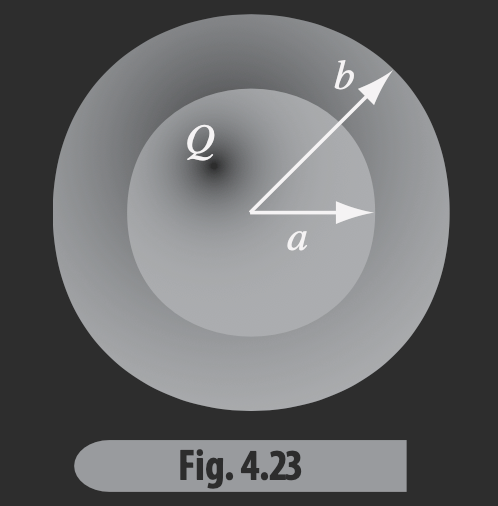
\includegraphics[width=0.3\linewidth]{fig4_23.png} & 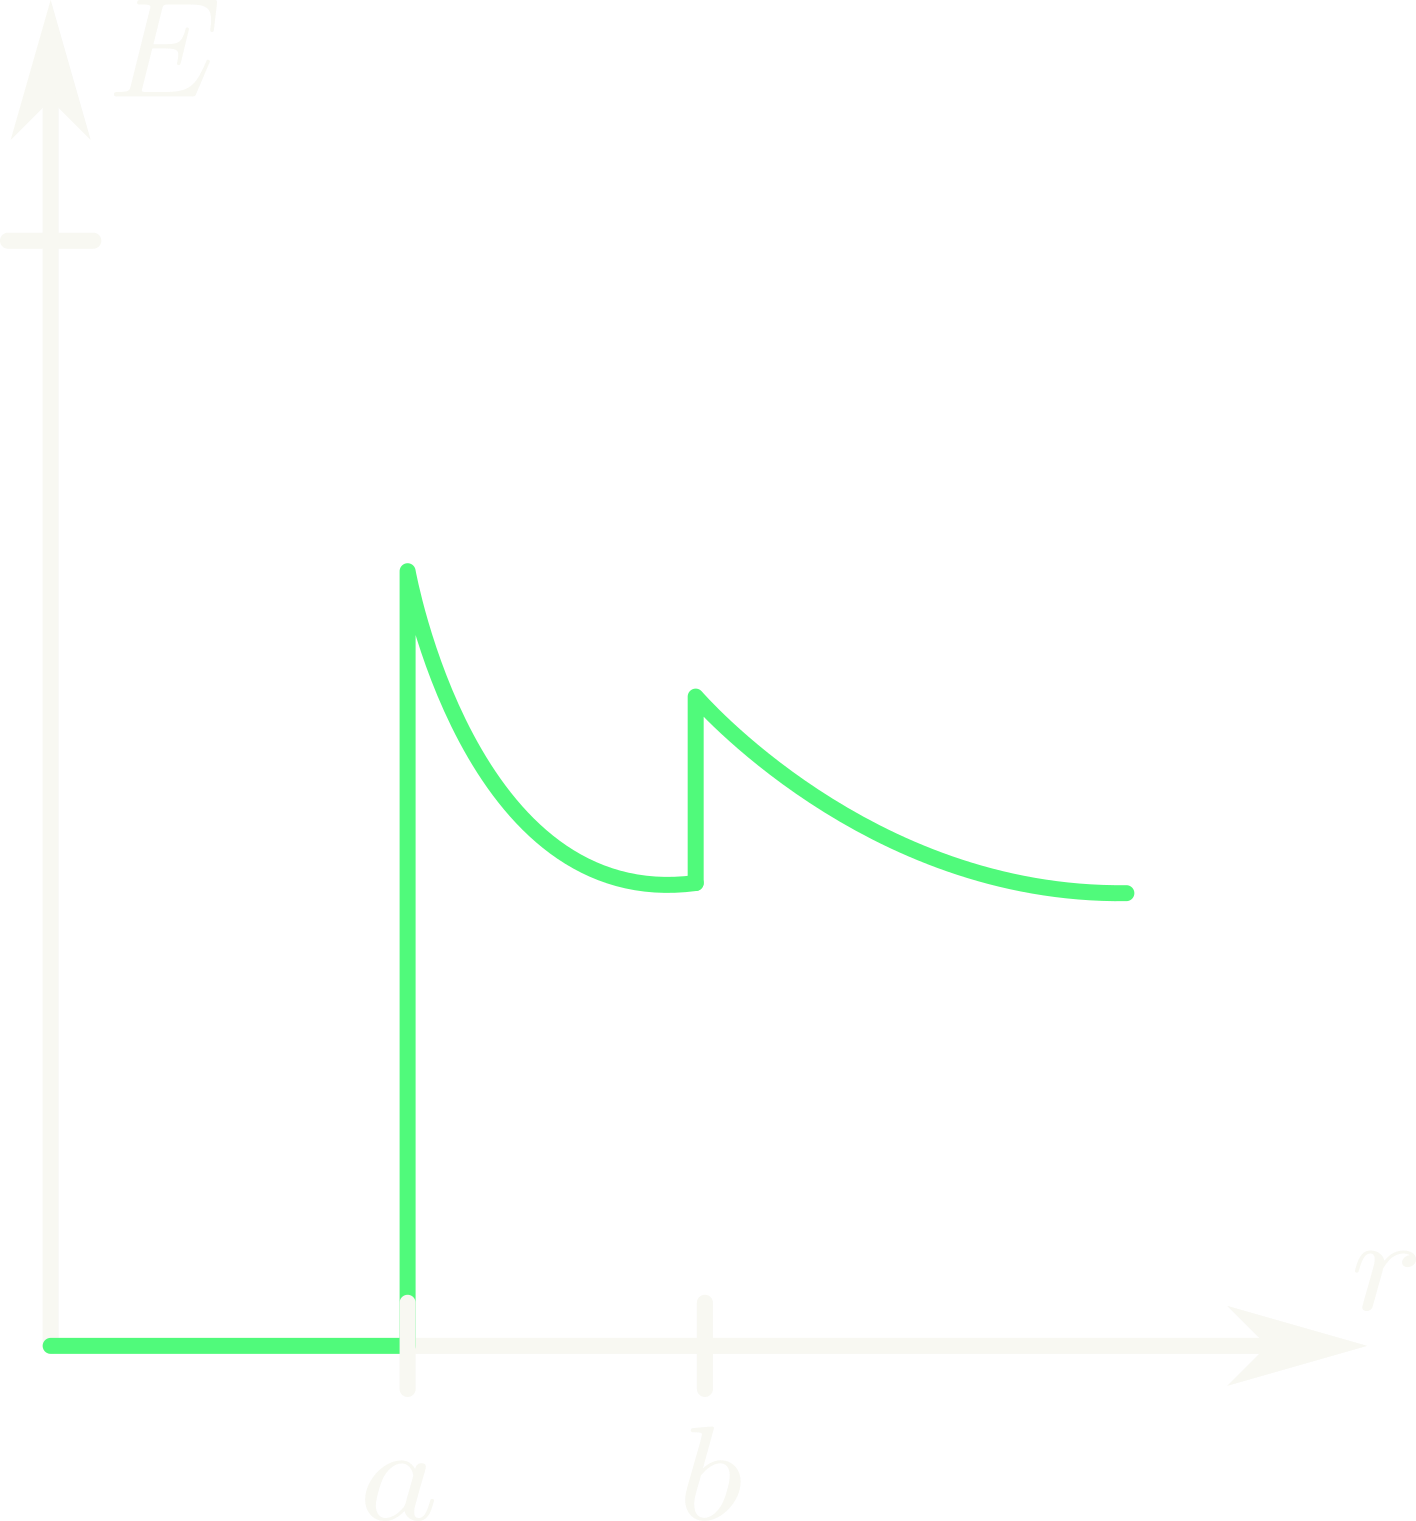
\includegraphics[width=0.3\linewidth]{fig4_23b.png} \\
        (a) & (b)
    \end{tabular}
    \caption{(a) Dielectric sphere surrounding metal sphere. (b) Electric field of resulting system.}
    \label{fig:4_23}
\end{figure*}

\newpage
\lhead{Lecture 13: 10/10/24}

\begin{figure*}[ht]
    \centering
    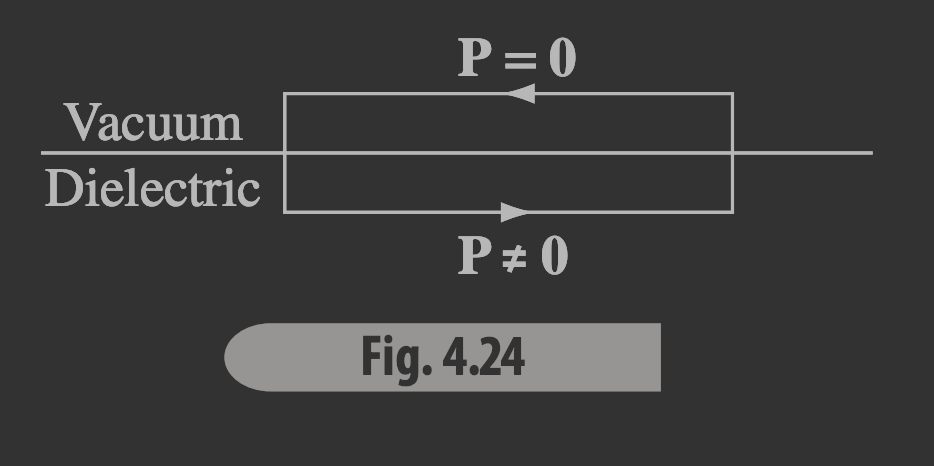
\includegraphics[width=0.5\linewidth]{fig4_24.png}
    \caption{Interface between polarized dielectric and vacuum.}
    \label{fig:4_24}
\end{figure*}

Since $\vb P$ is zero on the vacuum side but not on the dielectric side
\begin{align*}
    \oint \vb P \cdot \dd{\vb*\ell} \neq 0
\end{align*}
In addition, the displacement field $\vb D = \epsilon \vb E + \vb P$ implies
\begin{align*}
    \oint \vb D \cdot \dd{\vb a} \neq 0 \neq \curl \vb D
\end{align*}
Furthermore, the proportionality factor $\epsilon_0 \chi_e$ is different on both sides.
For the homogeneous linear dielectric
\begin{align*}
    \div \vb D = \rho_f \qand \curl \vb D = 0
\end{align*}
where 
\begin{align*}
    \begin{cases}
        \chi_f \vb E_\text{vac} = \ke \frac{q}{r^2} \\
        \chi_c \vb D = \ke \frac{q}{r^2}
    \end{cases}
    \implies \vb E = \epsilon \vb E
\end{align*}
or
\begin{align*}
    \vb E = \frac{1}{\epsilon} \vb D
\end{align*}

\paragraph{Example:} Parallel plate capacitor with insulating material of dielectric constant $\epsilon_r$
\begin{align*}
    \vb E \to \frac{\vb E}{\epsilon_r} 
\end{align*}
and the potential differnce between the plates is
\begin{align*}
    V = - \int \vb E \cdot \dd{\vb*\ell} = - Ed \to \frac{Ed}{\epsilon_r}
\end{align*}
And the capacitance is
\begin{align*}
    C = \frac{Q}{V} \to \frac{\epsilon_r Q}{V} = \epsilon_r C
\end{align*}

\subsubsection*{Boundary Value Problems with Linear Dielectrics}

From the given properties of the displacement vector
\begin{align*}
    \vb D &= \epsilon_0 \vb E + \vb P \\
    &= \epsilon_0 (1 + \chi_e) \vb E 
\end{align*}
where $\vb P = \epsilon_0 \chi_e \vb E$ so
\begin{align*}
    \vb D = \epsilon \vb E
\end{align*}
We can get the bound charge densities
\begin{align*}
    \rho_b = -\div \vb P = -\div(\frac{\epsilon_0 \chi_e}{\epsilon} \vb D), \quad \sigma_b = \vb P \cdot \vu n
\end{align*}
which implies
\begin{align*}
    \boxed{
        \rho_b = -\qt(\frac{\chi_e}{1 + \chi_e}) \rho_f
    }
\end{align*}
Since the net charge resides in the surface of the dielectric, i.e. $\rho = 0$ so from Laplace's equation
\begin{align*}
    \epsilon_\text{above} \vb E_\text{above}^\perp - \epsilon_\text{below} \vb E_\text{below}^\perp = \sigma_f
\end{align*}
or in terms of voltage (from $\vb E = -\grad V$)
\begin{align*}
    \epsilon_\text{above} \pdv{V_\text{above}}{n} - \epsilon_\text{below} \pdv{V_\text{below}}{n} = -\sigma_f
\end{align*}
And since the potential is still continuous
\begin{align*}
    V_\text{above} = V_\text{below}
\end{align*}

\paragraph{Example:} Sphere of homogeneous linear dielectric material in a uniform $\vb E_0$.
Find $\vb E$ in sphere.

\begin{figure*}[ht]
    \centering
    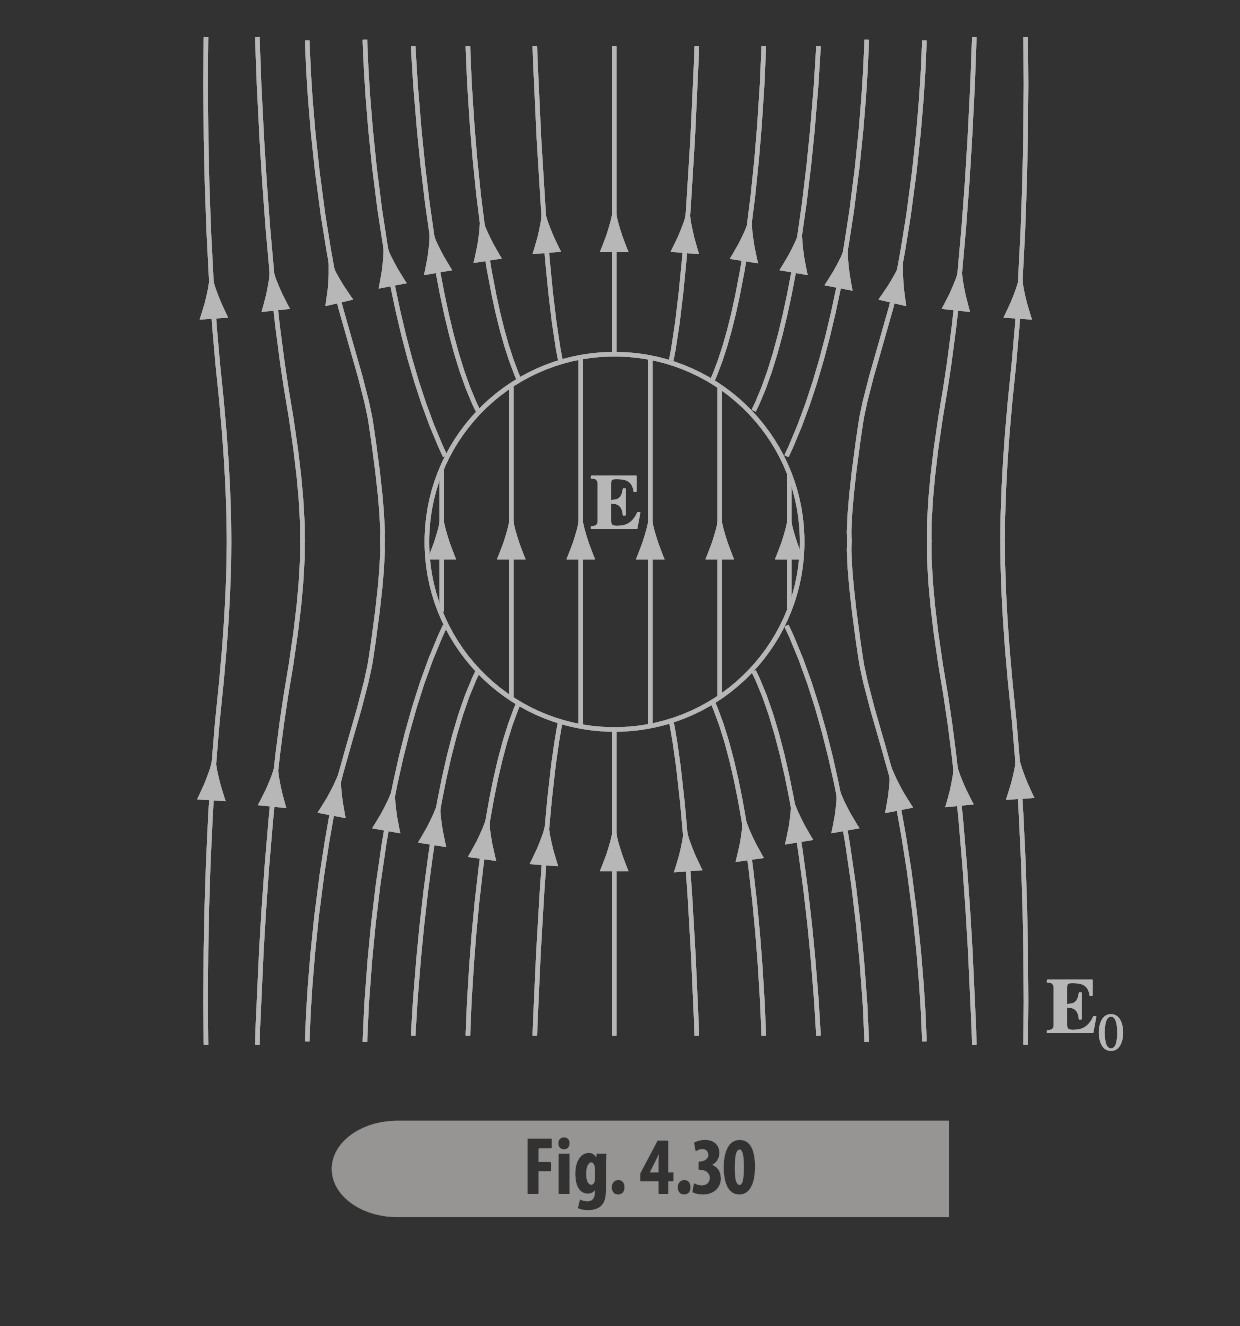
\includegraphics[width=0.3\linewidth]{fig4_30.png}
    \caption{Homogeneous linear dielectric sphere in uniform E-field $\vb E_0$.} 
    \label{fig:4_30}
\end{figure*}

Using B.C. to solve Laplace's equation
\begin{itemize}
    \item [(i)] $V_\text{in} = V_\text{out}$ at $r = R$
    \item [(ii)] $\epsilon \pdv{V_\text{in}}{r} = \epsilon_0 \pdv{V_\text{out}}{r}$ at $r = R$ where $\epsilon = \epsilon_0 \epsilon_r$
    \item [(iii)] $V_\text{out} = -E_0 r\cos\theta$ at $r \gg R$
\end{itemize}

From the Legendre polynomials
\begin{align*}
    V_\text{in} = \sum_{l = 0}^\infty A_l r^l P_l(\cos\theta)
\end{align*}
and outside the sphere
\begin{align*}
    V_\text{out} = \underbrace{-E_0 r \cos\theta}_\text{external field} + \underbrace{\sum_{l = 0}^\infty \frac{B_l}{r^{l + 1}} P_l(\cos\theta)}_\text{due to sphere} 
\end{align*}
and at $r = R \to V_\text{in} = V_\text{out}$ so
\begin{align*}
    \sum_l A_l R^l P_l(\cos\theta) = -E_0 R \cos\theta + \sum_l \frac{B_l}{R^{l + 1}} P_l(\cos\theta)
\end{align*}
Remembering that $P_0 = 1$ and $P_1 = \cos\theta$ we get from (i)
\begin{align*}
    \begin{cases}
        A_1 R = -\epsilon_0 R + \frac{B_1}{R^2} & l = 1 \\
        A_l R_l = \frac{B_l}{R^{l + 1}} & l \neq 1
    \end{cases}
\end{align*}
and from (ii) 
\begin{align*}
    \epsilon_r \sum_l A_l R^{l + 1} P_l (\cos\theta) = -\epsilon_0 \cos\theta
        - \sum_l \frac{(l + 1)B_l}{R^{l + 2}} P_l(\cos\theta)
\end{align*}
so the orthogonality of the Legendre polynomials gives
\begin{align*}
    \begin{cases}
        \epsilon_r A_1 = -\epsilon_0 - \frac{2B_1}{R^3} & l = 1 \\
        \epsilon_r l A_l R^{l - 1} = - \frac{(l + 1)B_l}{R^{l + 2}} & l \neq 1
    \end{cases}
\end{align*}
After staring at it for some time and looking through the math
\begin{align*}
    \begin{cases}
        A_l = B_l = 0 & l \neq 1 \\
        A_1 = -\frac{3}{\epsilon_r + 2} E_0 \qand B_1 = \frac{\epsilon_r - 1}{\epsilon_r + 2} R^3 E_0 & l = 1
    \end{cases}
\end{align*}
Thus the potentials are
\begin{align*}
    V_\text{in} (r, \theta) = -\frac{3\epsilon_0}{\epsilon_r + 2} r \cos\theta = -\frac{3\epsilon_0}{\epsilon_r + 2} z
\end{align*}
so the electric field is
\begin{align*}
    \vb E_\text{in} = -\grad V = \frac{3}{\epsilon_r + 2} \vb E_0
\end{align*}
The field inside the sphere will go to zero if the dielectric constant is infinite.

\paragraph{Another example:} Everything below plane $z = 0$ is linear dielectric with susceptibility $\chi_e$.
Calculating the force on a charge $q$ a distance $d$ above the origin.

\begin{figure*}[ht]
    \centering
    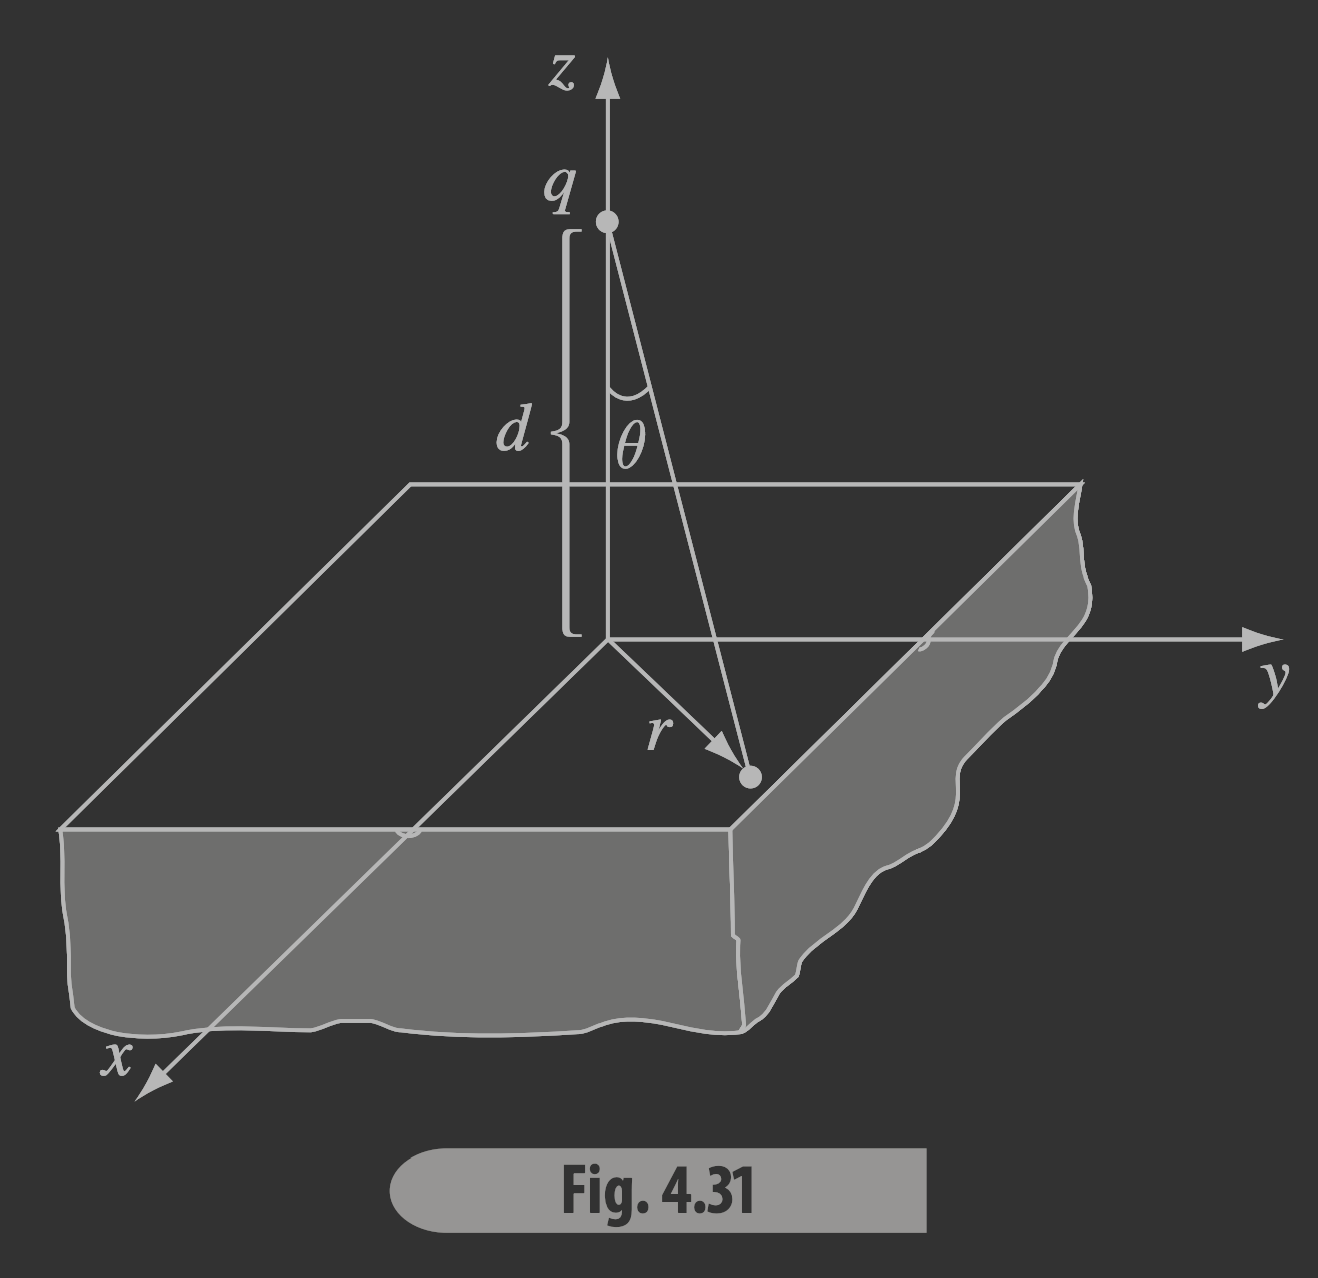
\includegraphics[width=0.3\linewidth]{fig4_31.png}
    \caption{Everything below $z = 0$ is a dielectric}
    \label{fig:4_31}
\end{figure*}

Earlier we found a relationship in the volume of a dielectric sphere being $\rho_b \propto \rho_f = 0$,
so we only need to worry about the bound surface charge density
\begin{align*}
    \sigma_b &= \vb P \cdot \vu n = P_z, \quad \vb P = \epsilon_0 \chi_e \vb E \\
    &= P_z = \epsilon_0 \chi_e E_z
\end{align*}
where $E_z$ is the $z$-component of the TOTAL field. The total field due to $q$ and $\sigma_b$:
\begin{itemize}
    \item $z$-comp of the charge $q$
    \begin{align*}
        E_q = -\ke \frac{q}{r^2 + d^2} \cos\theta = -\ke \frac{qd}{(r^2 + d^2)^{3/2}}
    \end{align*}
    \item $z$-comp of the bound surface charge
    \begin{align*}
        E_{\sigma_b} = -\frac{\sigma_b}{2\epsilon_0} 
    \end{align*}
\end{itemize}
So
\begin{align*}
    \sigma_b = \epsilon_0 \chi_e \qt[
        -\ke \frac{qd}{(r^2 + d^2)^{3/2}} - \frac{\sigma_b}{2\epsilon_0}
    ]
\end{align*}
and solving for $\sigma_b$ we get
\begin{align*}
    \sigma_b = -\frac{1}{2\pi} \qt(\frac{\chi_e}{\chi_e + 2}) \frac{qd}{(r^2 + d^2)^{3/2}}
\end{align*}
Which is exactly the same as the surface charge of an induced surface charge on an infinite conducting plane\dots

The total bound charge is therefore
\begin{align*}
    q_b = -\qt(\frac{\chi_e}{\chi_e + 2}) q
\end{align*}

\newpage
\lhead{Lecture 14: 10/15/24}

\subsubsection{Energy in Dielectrics}
The work it takes to charge a capacitor is
\begin{align*}
    W = \frac{1}{2} CV^2
\end{align*}
where the a capacitor filled with a linear dielectric has a capacitance
\begin{align*}
    C = \epsilon_r C_0
\end{align*}
Thus the energy stored in this system is
\begin{align*}
    W_\text{die} &= \frac{\epsilon_0} \int \epsilon_r E^2 \dd{\tau}
\end{align*}
and using $\vb D = \epsilon \vb E = \epsilon_0 \epsilon_r \vb E$ we get
\begin{align*}
    \boxed{
        W = \frac{1}{2} \int \vb D \cdot \vb E \dd{\tau}
    }
\end{align*}
which is integrated over all space.

\paragraph{Example} Sphere of radius $R$ filled with dielectric $\epsilon_r$ and free charge $\rho_f$ has energy (from Gauss's Law)
\begin{gather*}
    \oint D \cdot \dd{\vb a} = Q_{\text{f, enc}} \\
    \implies \vb D(\vb r) = \begin{cases}
        \dfrac{\rho_f}{3} \vb r & r < R \\
        \dfrac{\rho_f}{3} \dfrac{R^3}{r^2} \vb r & r > R
    \end{cases}
\end{gather*}
Thus the correlated E-field
\begin{align*}
    \vb E (\vb r) = \begin{cases}
        \dfrac{\rho_f}{3\epsilon_0 \epsilon_r} \vb r & r < R \\
        \dfrac{\rho_f}{3\epsilon_0 \epsilon_r} \dfrac{R^3}{r^2} \vb r & r > R
    \end{cases}
\end{align*}
The purely electrostatic energy is $W_\text{es} = \frac{\epsilon_0}{2} \int E^2 \dd{\tau}$ or
\begin{align*}
    W_\text{es} &= \frac{\epsilon_0}{2} \qt[
        \qt(\frac{\rho_f}{3 \epsilon_0 \epsilon_r})^2 \int_0^R r^2 (4\pi r^2) \dd{r}
        + \qt(\frac{\rho_f}{3 \epsilon_0})^2 R^6 \int_R^\infty \frac{1}{r^4} (4\pi r^2) \dd{r} 
    ] \\
    &= \frac{2\pi}{9\epsilon_0} \rho_f^2 R^5 \qt(\frac{1}{5\epsilon_r^2} + 1)
\end{align*}
but the total energy is
\begin{align*}
    W_\text{tot} &= \frac{1}{2} \int \vb D \cdot \vb E \dd{\tau} \\
    &= \frac{1}{2} \qt[
        \frac{\rho_f^2}{9 \epsilon_0 \epsilon_r} \int_0^R r^2 (4\pi r^2) \dd{r}
        + \qt(\frac{\rho_f}{3} R^3) \qt(\frac{\rho_f}{3\epsilon_0} R^3) \int_R^\infty \frac{1}{r^4} (4\pi r^2) \dd{r}
    ] \\
    &= \frac{2\pi}{9\epsilon_0} \rho_f^2 R^5 \qt(\frac{1}{5\epsilon_r} + 1)
\end{align*}
Thus 
\begin{align*}
    W_\text{es} < W_\text{tot} 
\end{align*}
So starting with the unpolarized dielectric sphere and using the ``method of assembly'' i.e. adding charge $\dd{q}$ to each layer of the sphere, we have the field in three regions
\begin{align*}
    \vb E(\vb r) = \begin{cases}
        \dfrac{\rho_f}{3\epsilon_0 \epsilon_r} \vb r & r < r' \\
        \dfrac{\rho_f}{3\epsilon_0 \epsilon_r} \dfrac{R^3}{r^2} \vb r & r' < r < R \\
        \dfrac{\rho_f}{3\epsilon_0} \dfrac{R^3}{r^2} \vb r & r > R
    \end{cases}
\end{align*}
And bringing down $\dd{q}$ from $\infty \to r'$ the infinitesimal work is
\begin{align*}
    \dd{W} &= -\dd{q} \qt[\int_\infty^R \vb E \cdot \dd{\vb l} + \int_R^{r'} \vb E \cdot \dd{\vb l}] \\
    &= -\dd{q} \qt[
        \frac{\rho_f r'^3}{3 \epsilon_0} \int_\infty^R \frac{1}{r^2} \dd{r} 
        + \frac{\rho_f r'^3}{3 \epsilon_0 \epsilon_r} \int_R^{r'} \frac{1}{r^2} \dd{r}
    ] \\
    &= \frac{\rho_f r'^3}{3\epsilon_0} \qt(
        \frac{1}{R} + \frac{1}{\epsilon_r} \qt(\frac{1}{r'} - \frac{1}{R})
    ) \dd{q} 
\end{align*}
which increases the radius by
\begin{align*}
    \dd{q} = \rho \dd{V} = \rho_f (4\pi'^2) \dd{r'}
\end{align*}
thus
\begin{align*}
    \dd{W} = \frac{\rho_f}{3\epsilon_0} \qt[
        \frac{r'^3}{R} \qt(1 - \frac{1}{\epsilon_r}) + \frac{r'^2}{\epsilon_r} 
    ] \dd{q}
\end{align*}
So the total work is done by integrating over $0 \to R$
\begin{align*}
    W &= \int \dd{W} = \int (\;) \dd{q} \to \int (\;) \dd{r'} \\
    &= \frac{4\pi \rho_f^2}{3\epsilon_0} \qt[
        \frac{1}{R} \qt(1 - \frac{1}{\epsilon_r}) \int_0^R r'^5 \dd{r'} + \frac{1}{\epsilon_r} \int_0^R r'^4 \dd{r'}
    ] \\
    &= \frac{2\pi}{9 \epsilon_0} \rho_f^3 R^5 \qt[
        \frac{1}{5\epsilon_r} + 1
    ] = W_\text{tot}
\end{align*}
So the energy of deformation is
\begin{align*}
    W_\text{def} = W_\text{tot} - W_\text{es} = \frac{2\pi}{45\epsilon_0 \epsilon_r^2} \rho_f^2 R^5 (\epsilon_r - 1)
\end{align*}
\paragraph{Another way\dots}
We can pretend that this deformation energy is analogous to a spring (separated by distance $d$ and spring constant $k$)
connecting two charges where one charge $+q$ is nailed down so 
\begin{align*}
    qE = kd
\end{align*}
here
\begin{align*}
    \vb E = \frac{\rho_f}{3\epsilon_0 \epsilon_r} \vb r \implies \qqtext{field of free charge, inside dielectric}
\end{align*}
thus the dipole $p = qd$ and polarization $P = p/ \dd{\tau}$. The spring constant and infinitesimal change in work is
\begin{align*}
    k &= \frac{\rho_f}{3\epsilon_0 \epsilon_r d^2} P r \dd{\tau} \\
    \dd{W} &= \frac{1}{2} kd^2 = \frac{\rho_f}{6\epsilon_0 \epsilon_r} P r \dd{\tau}
\end{align*}
This is will give us the energy stored in the dipole ``spring'' i.e.
\begin{align*}
    W_\text{sp} = \frac{\rho_f}{6\epsilon_0 \epsilon_r} \int P r \dd{\tau} 
\end{align*}
and the polarization is
\begin{align*}
    \vb P = \epsilon_0 (1 + \chi_e) \vb E = \epsilon_0 \chi_e \frac{\rho_f}{3\epsilon_0 \epsilon_r} \vb r = \frac{(\epsilon_r - 1) \rho_f}{3\epsilon_r} \vb r
\end{align*}
So
\begin{align*}
    W_\text{sp} &= \frac{\rho_f}{6\epsilon_0 \epsilon_r} \int \frac{(\epsilon_r - 1) \rho_f}{3\epsilon_r} (4\pi) \int_0^R r^4 \dd{r}  \\
    &= \frac{2\pi}{45\epsilon_0 \epsilon_r^2} \rho_f^2 R^5 (\epsilon_r - 1)
\end{align*}
which is the exact same thing! This is because our approximation for the polarization $\vb P = \epsilon_0 \chi_e \vb E$ is linear i.e. we were approximating for a spring the whole time!
\end{document}
